\section{Shock wave simulation}
We studied the evolution of moderately relativistic shocks and spectrum of accelerated particles. We chose relativistic shocks with a low Lorentz factor because the maximum energy of the produced cosmic rays increases with the shock wave Lorentz factor, while the efficiency of acceleration decreases, 
because it is more difficult for particle to cross fast moving front many times 
%
\cite{Ellison2013}. So we assume that the intermediate case of moderately relativistic shocks provides the most efficient acceleration.

We developed the implicit particle-in-cell (PIC) code, presented in our previous paper \cite{Romansky2016}, based on the scheme suggested by Lapenta et al.~\cite{Lapenta2006} and improved for the relativistic case by Noguchi et al.\cite{Noguchi2007}.
Our code is fully three-dimensional and parallelized with MPI technology, which is adapted for distributed computing and can be executed on a wide class of computers. We use 
%cleaning divergence of electric field 
the electric field divergence correction
after every several time steps and 
%Fourier filtering of shortwave harmonics 
the shortwave harmonics Fourier filtering
to suppress the numerical Cherenkov instability and improve the energy conservation.

In the modeling setup the homogeneous plasma flows in the simulation box through the right boundary
and collides with the reflecting superconducting wall on the left boundary, launching the shock wave. It is a common way to initialize a shock wave, because the initialization using the Rankine–Hugoniot conditions does not take into account the microscopic distribution, and the shock wave, created in such way, will probably fall apart into several discontinuities.

\begin{figure}[h!]
	\centering
	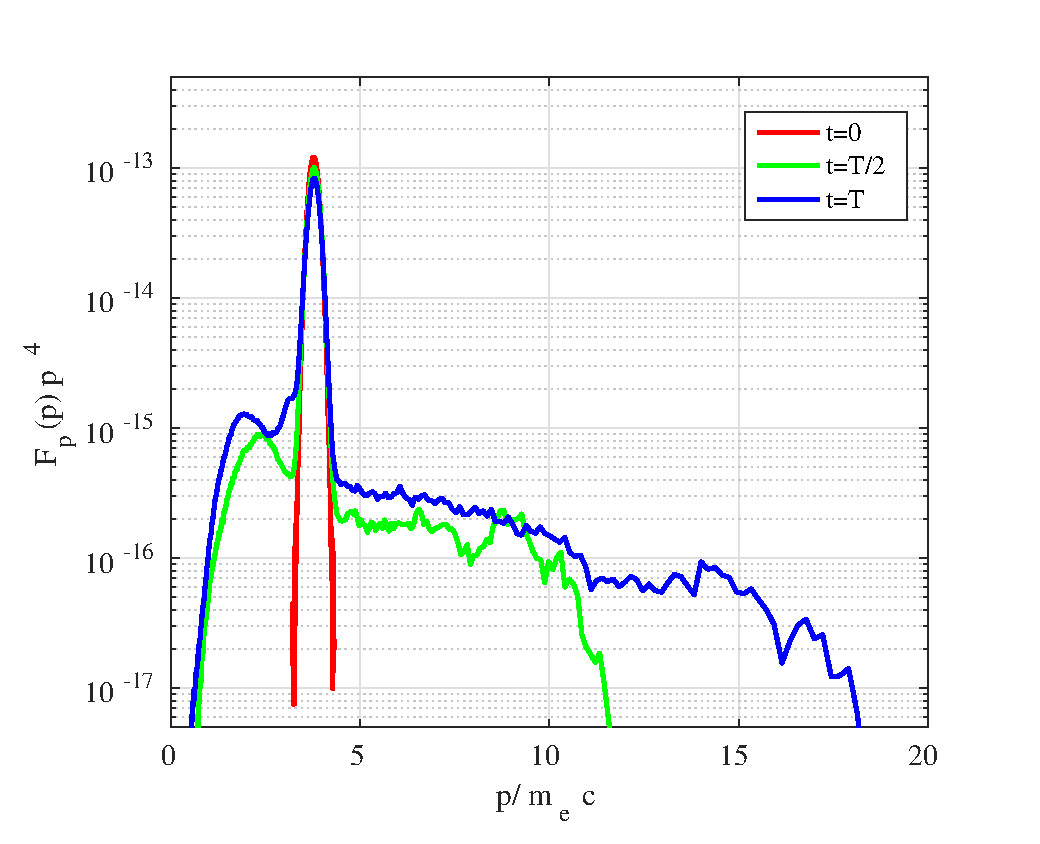
\includegraphics[width=1.0\textwidth]{fig/protons.eps} 
	\caption{Distribution of protons in the relativistic shock wave with Lorentz factor 1.5 with different inclination angle.}
	\label{protons}
\end{figure} 
  
The simulations are one-dimensional and have the following parameters: the initial flow Lorentz factor $\gamma = 1.5$, the number densities $n_e = 10^{-4} \rm{cm}^{-3}$, $n_p = 10^{-4} \rm{cm}^{-3}$ , the temperature $5\cdot10^8 \rm{K}$, the magnetic field $B = 10^{-4} \rm{G}$, the full size of the box $L = 2\cdot10^{12} \rm{cm}$, the number of cells $N=2\cdot10^4$. The electron mass is reduced to $m_e = \frac{m_p}{20}$. The full time of simulation is $T = 5000 {\omega_p}^{-1}$.This values gives the dimensionless parameter magnetization $\sigma = \frac{B^2}{4\pi\gamma (n_p m_p + n_e m_e) c^2} = 0.003$. Inclination angle $\theta$ is the angle between the flow velocity and the magnetic field. We present the results for the particle spectrum in several simulations with different $\theta$. The stable shock waves formed in all simulations and the total energy deviation is less than $3\%$, and it proves that our code provides correct model of the shock waves. 


\begin{figure}[h!]
	\centering
	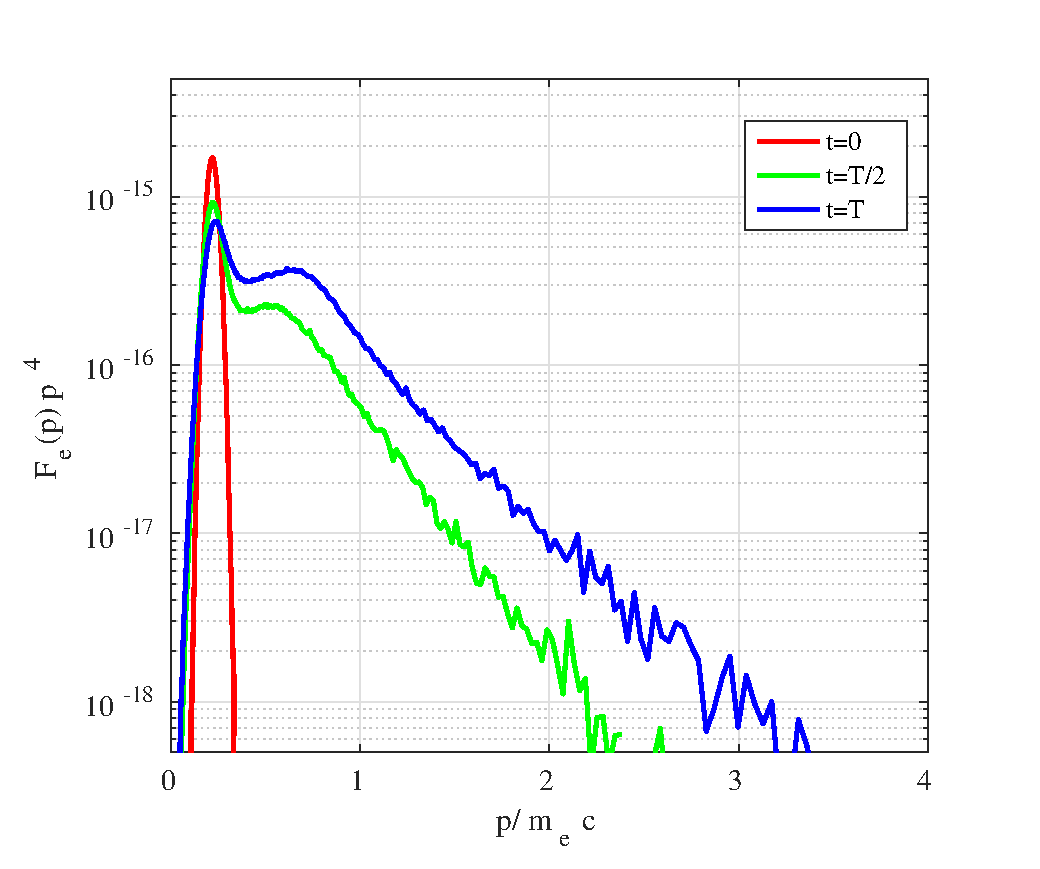
\includegraphics[width=1.0\textwidth]{fig/electrons.eps} 
	\caption{Distribution of electrons in the relativistic shock wave with Lorentz factor 1.5 with different inclination angle.}
	\label{electrons}
\end{figure}

One can see in Figures \ref{protons} and \ref{electrons} the particle spectrum for different angles $\theta$. The spectra consist of three parts - the narrow peak of cold but fast moving initial flow, the wide peak of hot downstream and the non-thermal accelerated component. Figures show that the spectrum of accelerated particles strongly depends on angle $\theta$. If $\theta$ is less than critical value, defined by the equation $c\cdot \cos(\theta_{crit})=v_{shock}$, where all values are measured in the upstream rest frame, particles can escape from the front and cross it several times to gain more energy (see, e.g., \cite{Pelletier2017}). It is difficult to evaluate the critical angle a priori, because the compression relation of the shock wave which will be created in the simulation is unknown. However the estimation for case of a strong wave (the compression relation equals $4$) provides $\theta_{crit}=45^{\circ}$ in the downstream frame, which is consistent with the results of our simulations.

Also, one can see that for the angles less then the critical one, the particle spectra are higher and longer for larger $\theta$. The spectrum of non-thermal component is about 10 times higher for protons than for electrons at the same energy. It is consistent with other Particle-in-cell simulations of the shock waves {\cite{Sironi2011}}.

The results show some interesting effects for angles close to the critical value (black and yellow lines)- electrons are still accelerating while protons are not. It can be explained by electrons acceleration in the short-wavelength turbulence of the shock wave precursor. Due to the small gyroradius of electrons in initial flow, short-wavelength turbulence scatter them more efficiently than protons. However, further research is necessary in order to study this phenomena in detail.



